\documentclass{article}

\usepackage{graphicx} % Required for inserting images
\usepackage{fancyhdr}
\usepackage{minted}
\usepackage{amsmath}
\usepackage{hyperref}
\usepackage{listings}
\usepackage{graphicx}
\usepackage[table,xcdraw]{xcolor}

\usepackage[
    a4paper,
    left=1in,
    right=1in,
    top=0.75in,
    bottom=0.75in
]{geometry}


\hypersetup{
    colorlinks=true,   % Farben statt Umrandung für Links
    linkcolor=black,    % Farbe für interne Links
    citecolor=blue,    % Farbe für Zitate
    filecolor=blue,    % Farbe für Dateien
    urlcolor=blue      % Farbe für URLs
}


\usepackage{array}
\pagestyle{fancy}
\title{Topic 2: Read Simulator}
\author{.}
\date{November 2024}


\begin{document}

    \maketitle
    \hrule
    \tableofcontents
    \vspace{10pt} % Optional: Add space after the TOC as well
    \hrule
    \renewcommand{\abstractname}{}

    \begin{abstract}
        \large
        RNA sequencing (RNAseq) is an important tool in transcriptomics, providing insights into gene expression, alternative splicing, and transcript discovery. Simulating RNAseq reads is essential for benchmarking computational tools under controlled conditions. This study outlines a robust simulation pipeline that fragments transcriptomic regions, generates paired-end reads with mutations to mimic sequencing errors, and maps these reads back to a reference genome. Key components include optimized GTF parsing for transcript extraction, a Gaussian-based fragment length sampling, and an efficient FASTA indexing mechanism for sequence retrieval. Performance and correctness were validated through rigorous tests on sequence extraction, genomic position mapping, and mutation distribution. Simulations exhibited linear runtime scalability relative to read count, highlighting the system’s efficiency for large datasets. Detailed visual and statistical analyses of mutation patterns, fragment lengths, and read distributions demonstrated the simulator’s fidelity.
    \end{abstract}


    \pagebreak


    \section{Introduction}
    \maketitle
    RNA sequencing (RNAseq) is a powerful and widely used method for analyzing the transcriptome, providing insights into gene expression patterns, alternative splicing, and discovering novel transcripts. By converting RNA into complementary DNA (cDNA) and sequencing it using high-throughput platforms, researchers can quantify and characterize the complete set of RNA transcripts present in a sample. The results of an RNAseq experiment are a set of sequenced reads in the FASTQ format (either single-end or paired-end). These reads are then mapped back onto the reference genome using a mapper like \texttt{Segemehl}.

    Accurate simulation of RNAseq reads is essential for benchmarking computational tools and testing hypotheses under controlled conditions. The task involves selecting specific genomic or transcriptomic regions from a genome FASTA file and simulating random fragmentation of these sequences. These fragments are then "sequenced" from both the forward and reverse strands, incorporating random point mutations to mimic sequencing errors. The result is a simulated dataset that closely resembles actual RNAseq data, providing a controlled environment to benchmark mapping tools by comparing known origin positions of reads with those predicted by the mapper. Figure \ref{fig:read-diagraml} shows an example of a paired-end read on a fragment and how it is mapped back onto the genome. By utilizing this approach, we can validate the mapper since we know the origin of the reads. Further analysis of the results may provide insights into areas where the mapper performs poorly, such as with split reads that only include a short section of an exon, as will be discussed later. It is important to note that a simulator cannot perfectly replicate an actual experiment; it relies on approximations and simplifications, such as using a uniform mutation rate per base (as discussed later) or employing a normal distribution to sample fragment lengths.

    \begin{figure}
        \centering
        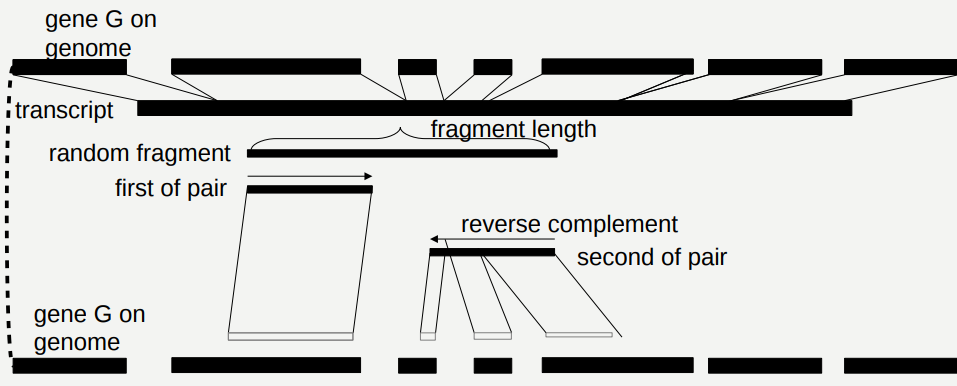
\includegraphics[width=1.0\textwidth]{figures/readsimulator/readdiagram.png}
        \caption{Example of an RNAseq paired-end read}
        \label{fig:read-diagraml}
    \end{figure}


    \section{Program Structure}

    \subsection{Program Usage}
    \begin{verbatim}
usage: java -jar readsimulator.jar [-h] -length <read length>
                           -frlength <mean fragment length>
                           -SD <standard deviation>
                           -readcounts <read counts file>
                           -mutationrate <mutation rate>
                           -fasta <genome FASTA file>
                           -fidx <genome FASTA file index>
                           -gtf <annotation file> -od <output directory>
                           [-analysis-script <path-to-script>]

named arguments:
  -h, --help             show this help message and exit
  -length <read length>  readsimulator.Read length
  -frlength <mean fragment length>
                         Mean fragment length
  -SD <standard deviation>
                         Standard deviation of fragment length
  -readcounts <read counts file>
                         Path to read counts file
  -mutationrate <mutation rate>
                         Mutation rate in percent. Between 0.0 and 100.0
  -fasta <genome FASTA file>
                         Path to genome FASTA file
  -fidx <genome FASTA file index>
                         Path to genome FASTA file index
  -gtf <annotation file>
                         Path to annotation file
  -od <output directory>
                         Output directory
  -analysis-script <path-to-script>
                         Path to the analysis  file  to analyze the results
                         directly
    \end{verbatim}

    \subsection{Program Procedure}
    The general structure of the program is as follows:

    \begin{enumerate}
        \item \textbf{Initialization and Setup}: Creation of the \texttt{ReadSimulator} object, which initializes the annotation, the \texttt{GenomeSequenceExtractor}, and the parameters for the simulation.
        \item \textbf{Read Simulation Process}:
        \begin{enumerate}
            \item \textbf{Iterate Through Read Counts}: The program iterates over the read counts specified for simulation.
            \item \textbf{Transcript Sequence Extraction}: Extract the complete transcript sequence using the \texttt{GenomeSequenceExtractor}.
            \item \textbf{Read Creation}:
            \begin{enumerate}
                \item \textbf{Fragment Length Sampling and Positioning}: Randomly sample the fragment length and determine the starting position on the transcript.
                \item \textbf{Read Pair Creation}: Generate a read pair based on the sampled fragment length and positions.
                \item \textbf{Mutation of Reads}: Introduce mutations to the read pairs as the simulation parameters specify.
                \item \textbf{Genomic Position Calculation}: Calculate the genomic positions of the reads, mapping them back to the original genomic coordinates.
                \item \textbf{Writing Results}: Use buffered output to write the read pairs to the mapping and FASTQ files, ensuring efficient data handling.
            \end{enumerate}
        \end{enumerate}
    \end{enumerate}
    During initialization, the readcounts file is loaded. The \texttt{readCountsFile} method is designed to parse a read counts file structured in a tab-separated format, where each line contains a gene ID, a transcript ID, and a corresponding count of reads. The general process is as follows:

    \begin{enumerate}
        \item \textbf{Initialization}: A \texttt{HashMap} is created to store the gene-transcript counts, where each gene ID maps to another \texttt{HashMap} that holds transcript IDs and their associated counts.

        \item \textbf{File Reading}: The method uses a \texttt{BufferedReader} to read the file line by line, skipping the header line.

        \item \textbf{Line Parsing}: For each subsequent line:
        \begin{itemize}
            \item The method identifies the positions of the tab characters to separate the gene ID, transcript ID, and count.
            \item If the line is malformed (i.e., does not contain the expected number of tabs), it is skipped.
        \end{itemize}

        \item \textbf{Data Storage}: Valid entries are extracted and stored in the nested \texttt{HashMap}. The outer map uses the gene ID as the key, while the inner map uses the transcript ID as the key and the count as the value.

    \end{enumerate}


    During the initialization of the ReadSimulator, the GTF annotation is created using the same procedure as the Exon Skipping Program. However, an important optimization was implemented: rather than including all genes and transcripts, the GTF file is filtered to only include those relevant to the read simulation. Before processing a line, we begin by checking the attributes section to see if the gene ID exists in the readcounts hashmap. If it does not, we exit; otherwise, we proceed to check the transcript ID to determine if it is also in our hashmap. The line is only processed if both of these conditions are met. This filtering process led to a significant performance improvement during local testing, reducing processing time from approximately 5 seconds to around 2 seconds. However, on the submission server, this optimization resulted in only a modest improvement of 0.5 seconds. If a large number of genes and transcripts are being simulated, this filtering step might add unnecessary complexity and could be omitted to streamline the process.

    A FASTA index file (often with a \texttt{.fai} extension) is a companion file to a FASTA sequence file. It provides a way to quickly access specific sequences within the FASTA file without needing to read the entire file. Each entry in the index corresponds to a sequence in the FASTA file and typically includes:
    \begin{itemize}
        \item \textbf{Chromosome/Sequence Name:} The identifier for the sequence.
        \item \textbf{Byte Offset:} The position in the FASTA file where the sequence starts.
        \item \textbf{Line Bases:} The number of bases (nucleotides) per line in the FASTA file.
        \item \textbf{Line Bytes:} The number of bytes used for each line, including any newline characters.
        \item \textbf{Length:} The total length of the sequence.
    \end{itemize}
    This structure allows the program to jump directly to the relevant part of the FASTA file, enabling efficient retrieval of sequence data, especially useful for large genomic datasets.

    The \texttt{FastaIndexEntry} class is defined as follows:
    \begin{verbatim}
private record FastaIndexEntry(long byteOffset, int lineBases, int lineBytes, int length) {}
    \end{verbatim}
    This class serves as a simple data structure to store the information retrieved from the FASTA index file. Its components include:
    \begin{itemize}
        \item \textbf{byteOffset:} Indicates where the sequence starts in the FASTA file, allowing direct access.
        \item \textbf{lineBases:} Specifies how many bases are present in each line, aiding in reading the sequence correctly.
        \item \textbf{lineBytes:} Represents the total number of bytes used for each line, crucial for accurate mapping.
        \item \textbf{length:} Indicates the total length of the sequence, useful for validation.
    \end{itemize}

    In the \texttt{GenomeSequenceExtractor} class, the following is defined:
    \begin{verbatim}
public class GenomeSequenceExtractor {
    private final FileChannel fileChannel;
    private final Map<String, FastaIndexEntry> fastaIndex;
}
    \end{verbatim}
    Here:
    \begin{itemize}
        \item \textbf{fileChannel:} Used to read from the FASTA file, allowing efficient file operations.
        \item \textbf{fastaIndex:} Stores the index entries for each chromosome, enabling quick lookups for specific sequences.
    \end{itemize}

    The method \texttt{readSequenceForExonsInOneRead} retrieves the entire genomic sequence that spans the specified exons, calculated from the first and last exons in the \texttt{TreeSet}. The \texttt{readSequence} method utilizes the FASTA index to locate the byte offset for the specified chromosome, providing essential information for mapping genomic data. The byte offset is calculated using the formula:
    \[
        \text{byteOffset} = \text{entry.byteOffset()} + \left(\frac{\text{start} - 1}{\text{entry.lineBases()}}\right) \times \text{entry.lineBytes()} + \left(\text{start} - 1\text{mod entry.lineBases()}\right)
    \]
    A \texttt{MappedByteBuffer} is created to read the sequence data directly from the file, minimizing I/O operations by mapping the required portion into memory. The code iterates through the \texttt{exons} to extract relevant portions, appending them to a \texttt{StringBuilder} to yield a final sequence containing only the exons.
% Talk more about extraction and when reverse is taken, how the index file works
    The transcript sequence is extracted using a MappedByteBuffer to retrieve the entire sequence from the transcript from start to end. Afterward, introns are removed to yield the final exon-only sequence. This approach is designed to minimize I/O operations. The fragment length is drawn using the \texttt{nextGaussian()} method from \texttt{SplittableRandom}. Instead of taking a maximum of the sampled fragment length and the read length, the fragment length is drawn until it is smaller than the transcript sequence and at least as long as the read length. While this approach results in more sampling, it provides greater accuracy, preventing an unusually high number of fragments from being clustered at the read length of 75. When generating reverse reads, rather than calculating the reverse complement for each individual reverse read sequence, it is more efficient to take the reverse complement of the entire transcript sequence at once. This approach is advantageous because when creating numerous reads from a single transcript, you end up calculating the reverse complement of the same transcript section multiple times.
    When modeling the occurrence of mutations across a fixed number of positions (e.g., 75 positions) with a given mutation rate, the situation can be represented by a binomial distribution. In this case, each position can either mutate or not mutate, with the probability of mutation defined by the mutation rate. The binomial distribution is characterized by two parameters: the number of trials ($n$) and the probability of success ($p$). Here, $n$ corresponds to the number of positions (75), and $p$ is the mutation rate (0.01).

    However, when the number of trials is large and the probability of success is small (which is often the case in biological contexts), the binomial distribution can be approximated by a Poisson distribution. The Poisson distribution is defined by a single parameter $\lambda$, which represents the average number of events (mutations) in a fixed interval. In this context, $\lambda$ can be calculated as:

    $$\lambda = n \cdot p$$

    In this implementation, the parameter $L$ is defined as:

    $$L = e^{-\lambda} = e^{-(\text{mutationRate} \cdot \text{readLength})}$$

    This value represents the probability of observing zero mutations in the sampled positions.


    The method \texttt{samplePoisson()} utilizes a common technique for sampling from a Poisson distribution. The algorithm works by generating random numbers until the cumulative product of these random numbers falls below the threshold $L$. Each iteration corresponds to a potential mutation event, and the process continues until the condition $p > L$ is no longer satisfied. The number of iterations ($k$) gives the total number of mutations sampled.

    This approach is computationally efficient because it avoids the need to calculate sample $n$ random numbers, which is what is needed to sample a binomial distribution. Once the number of mutations is determined, the \texttt{mutate()} method applies these mutations to the sequence. It randomly selects and modifies positions in the sequence, ensuring that each position is mutated only once. This process is efficient and straightforward, as it directly manipulates the sequence based on the sampled mutation count.


    The method \texttt{getCoveredRegion} identifies genomic coordinates by examining the exons of a transcript in relation to a specified region (\texttt{localRegion}). The process includes:

    \begin{enumerate}
        \item \textbf{Overlap Detection}: The method iterates through each exon to check for overlaps with the \texttt{localRegion}.
        \item \textbf{Coverage Calculation}: For each overlapping exon, it calculates the start and end positions of the covered region based on the boundaries of both the exon and the local region.
        \item \textbf{Result Compilation}: The calculated intervals are collected and returned, providing the genomic coordinates corresponding to the specified region.
    \end{enumerate}





    However, the process is more complex for genes on the reverse strand. This is because if a fragment starts at the first position of the transcript sequence, it actually corresponds to the last position of the last exon. An elegant trick is applied to correctly calculate the genomic coordinates for these reads (as seen in Figure \ref{fig:overlap-reverse-trick}. The transcript coordinates are effectively “shifted” by adjusting the read’s starting position. This means that the distance from the start of the read to the start of the transcript is now mapped to the distance from the end of the read to the end of the transcript. With this simple trick, the genomic coordinates are accurately calculated without needing to modify the \texttt{getCoveredRegion()} method itself.

    To reduce memory usage, the generated reads are written directly to the output file as they are produced rather than being collected in a list and printed at the end. This approach minimizes memory usage, especially when simulating large amounts of reads. To optimize I/O performance, a BufferedWriter is used, ensuring that writes to the file are not overly taxing. The BufferedWriter waits until its buffer is full before performing the actual write operation, which helps to efficiently manage I/O and improve performance.



    \begin{figure}
        \centering
        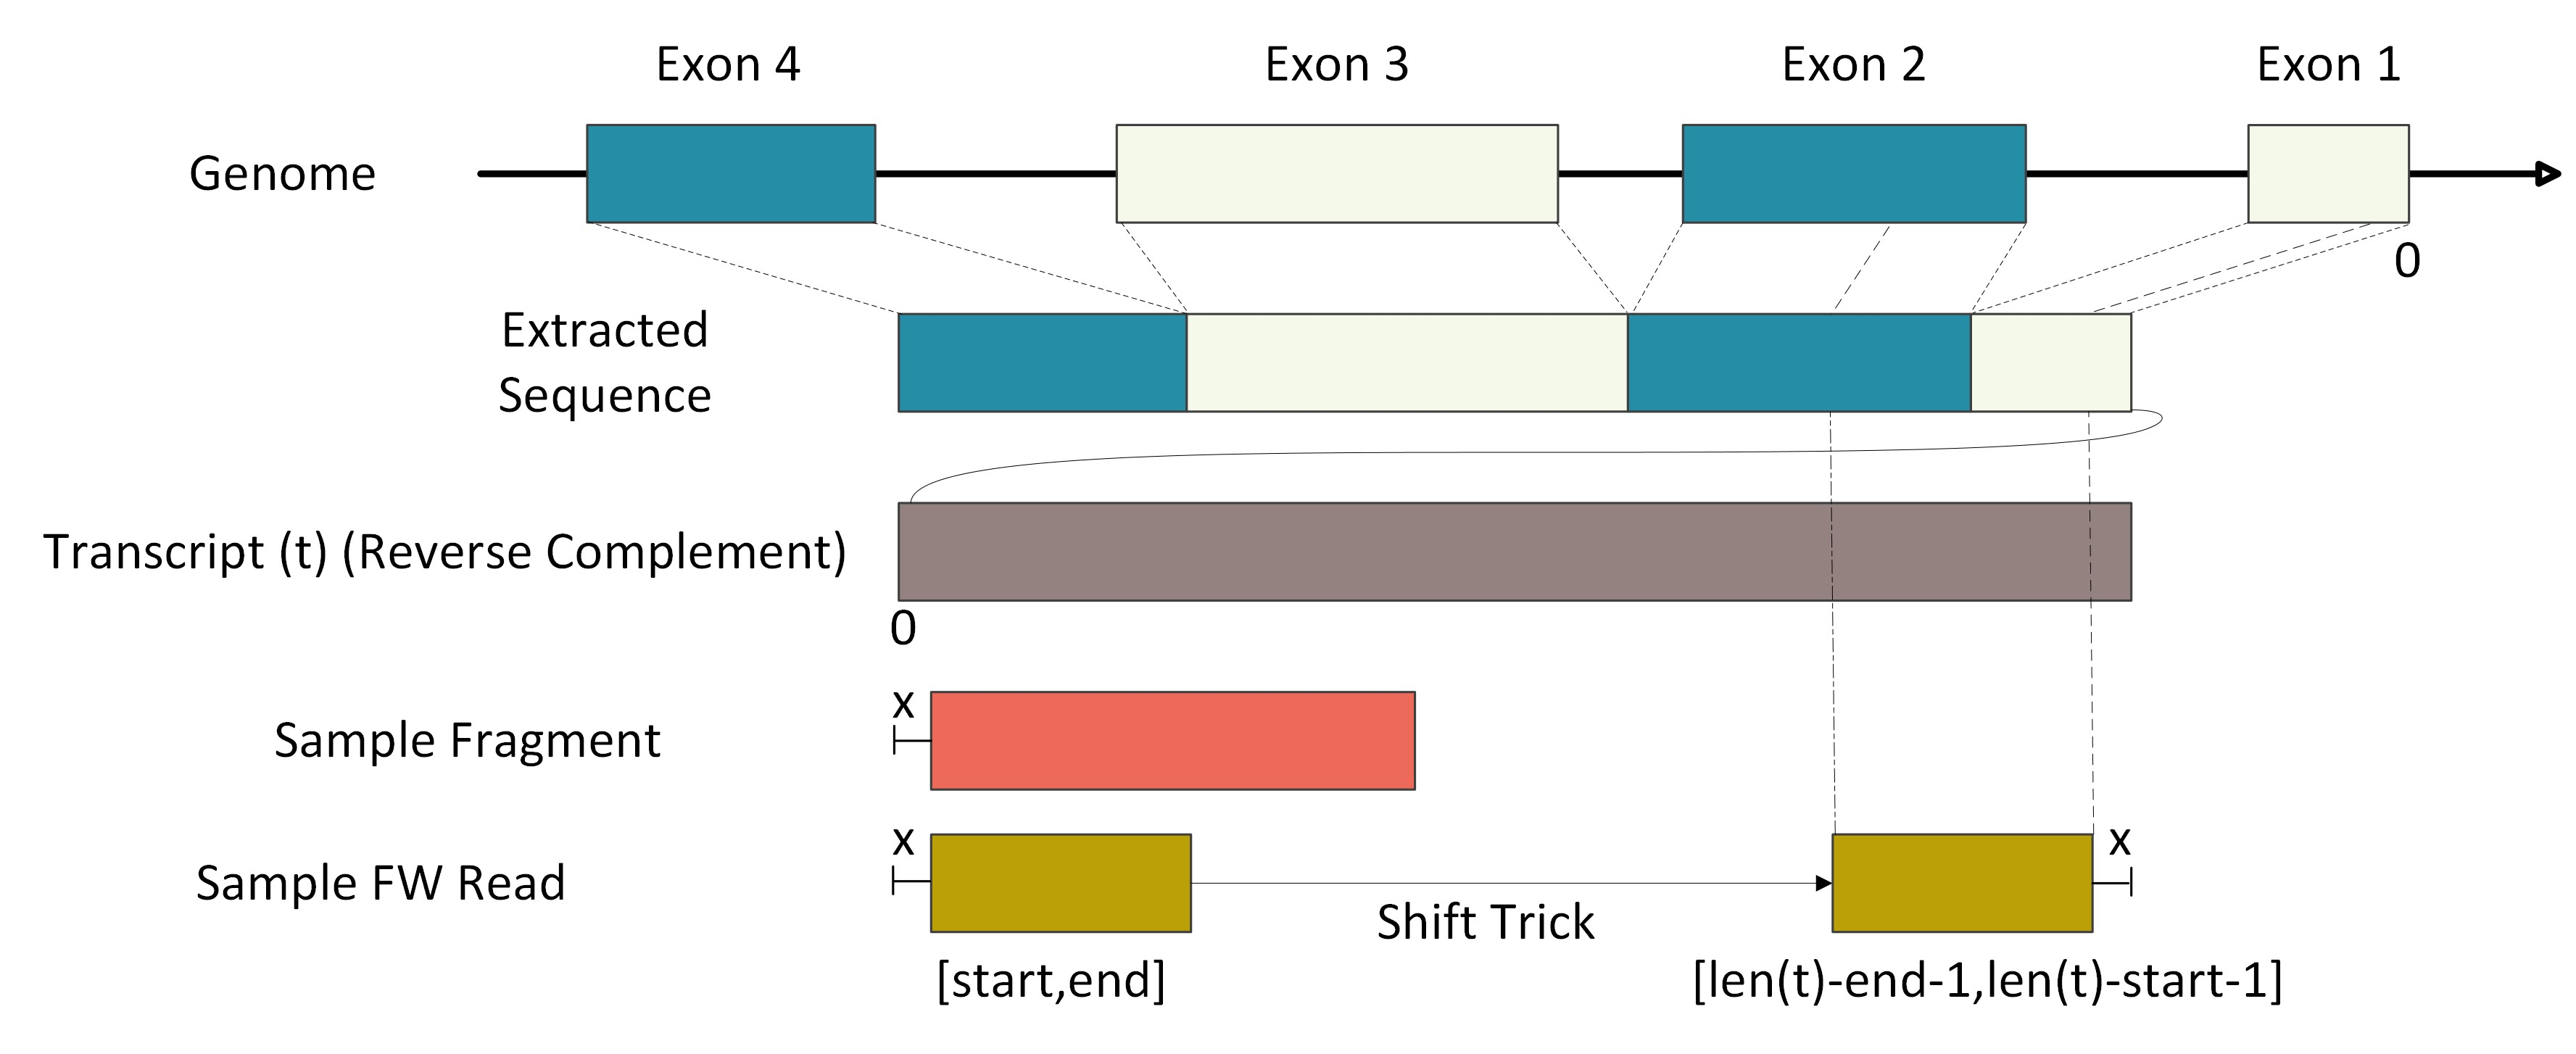
\includegraphics[width=1\textwidth]{figures/readsimulator/ReadSimulatorTrick.jpeg}
        \caption{Diagram showing trick used to calculate the genomic coordinates for reverse strand genes}
        \label{fig:overlap-reverse-trick}
    \end{figure}

    \subsection{Output Format}
    The program generates three output files: the \textbf{Read Mapping File}, the \textbf{Forward Reads}, and the \textbf{Reverse Reads}.

    \subsubsection{Read Mapping File}
    The \textbf{Read Mapping File} provides information about each read pair, with one line per pair. Each line consists of the following columns:

    \begin{itemize}
        \item \textbf{readid}: Integer identifier for the read pair, starting from 0.
        \item \textbf{chr id}: Chromosome ID.
        \item \textbf{gene id}: Gene ID.
        \item \textbf{transcript id}: Transcript ID.
        \item \textbf{fw regvec}: Genomic region vector for the forward read (1-based, end-exclusive).
        \item \textbf{rw regvec}: Genomic region vector for the reverse read (1-based, end-exclusive).
        \item \textbf{t fw regvec}: Region vector for the forward read in transcript coordinates (0-based, end-exclusive).
        \item \textbf{t rw regvec}: Region vector for the reverse read in transcript coordinates (0-based, end-exclusive).
        \item \textbf{fw mut}: Mutated positions in the forward read, represented as a comma-separated list of integers.
        \item \textbf{rw mut}: Mutated positions in the reverse read, represented as a comma-separated list of integers.
    \end{itemize}

    \subsubsection{FASTQ Reads}
    The forward and reverse reads are stored in FASTQ format. Each read in a FASTQ file consists of four lines:

    \begin{enumerate}
        \item \textbf{Header}: Begins with the '@' character, followed by the read ID.
        \item \textbf{Sequence}: The raw sequence of nucleotides.
        \item \textbf{Separator}: Begins with the '+' character, followed by the read ID (optional, but included for consistency).
        \item \textbf{Quality Scores}: A string encoding quality values for the sequence, with one symbol per nucleotide. In this program, all quality values are set to 'I', representing the maximum quality score.
    \end{enumerate}


    \section{Analysis}
    The analysis was performed with the sample files provided:
    \begin{itemize}
        \item \textbf{FASTA}: \textit{Homo\_sapiens.GRCh37.75.dna.toplevel.fa}
        \item \textbf{FASTA Index}: \textit{Homo\_sapiens.GRCh37.75.dna.toplevel.fa.fai}
        \item \textbf{GTF}: \textit{Homo\_sapiens.GRCh37.75.gtf}
        \item \textbf{Readcounts}: \textit{readcounts.simulation}

    \end{itemize}
    The program was run with the following parameters:
    \begin{verbatim}
java -jar readsimulator.jar
    -length 75
    -frlength 200
    -SD 80
    -mutationrate 1.0
    -gtf "./data/readsimulator/Homo_sapiens.GRCh37.75.gtf"
    -fasta "./data/readsimulator/Homo_sapiens.GRCh37.75.dna.toplevel.fa"
    -fidx "./data/readsimulator/Homo_sapiens.GRCh37.75.dna.toplevel.fa.fai"
    -readcounts "./data/readsimulator/readcounts.simulation"
    -od "./data/readsimulator/output"
    \end{verbatim}

% anaylsis of readcounts file

    \subsection{Correctness}
    Two JUnit tests were implemented to ensure the correctness of key components:
    \begin{itemize}
        \item The first test verifies that transcript sequence files are accurately read and processed by the \texttt{GenomeSequenceExtractor}.
        \item The second test checks the correctness of the genomic position calculations, ensuring the reads are correctly mapped to their original genomic locations.
    \end{itemize}

    \subsubsection{Sequence Extraction Test}
    A sample transcriptome (\textit{Homo\_sapiens.GRCh37.75.cdna.all.fa.gz}) was provided in a compressed form. This was read line by line as a \texttt{GZIPInputStream} and processed. The ID line was processed to extract the gene ID and transcript ID. The GTF Annotation was used to get the exon positions and extract the sequence using the \texttt{GenomeSequenceExtractor}. This sequence was tested against the sequence from the transcriptome. All transcriptome sequences (180,253) are read out correctly.

    \subsubsection{Genomic Position Test}
    To verify the accuracy of genomic coordinate extraction, this test replicates the read simulation process (as described before) using a sample input file, \texttt{readcounts.simulation}. Once reads are generated, mutated, and their genomic coordinates extracted, we retrieve the sequences from the reference FASTA file using the computed coordinates. This extraction uses a previously validated method to ensure correctness. We then compare the extracted sequences with the original simulated sequences to check for consistency. Additionally, we confirm that all genomic coordinates for the generated reads are correctly extracted.

    When optimizing the program for performance, this testing suite helps verify that improvements do not compromise correctness. By running these tests after performance-related modifications, we ensure that the accuracy of genomic coordinate extraction and mutation processes remains intact, ensuring that the core functionality of the simulator is preserved.

    \subsubsection{Mutation Rate}

    In addition to checking whether the mutated positions are actually mutated, the distribution of mutations can be analyzed to determine if the mutation rate is being applied correctly. In our sample run, a mutation rate of 1\% and read length of 75 was used. This corresponds to a Binomial Distribution with the parameters \(n=75, p=0.01\), as each position in the read has a 1\% chance of mutating. The mutation process can be modeled as a sequence of independent trials, where each trial represents a nucleotide, and the mutation probability is constant, thus following a binomial distribution. Figure \ref{fig:cumulative-distribution-mutation-counts} shows the distribution of the mutation counts of reads. As mentioned previously, to speed up the sampling process, the binomial distribution is approximated with a Poisson distribution but still matches a binomial CDF almost perfectly. The overlaid Binomial CDF matches our CDF, which shows the correctness of the implementation of the mutation calculation. Most reads have no or only have a very small amount of mutations, which is to be expected with a mutation rate of 1\%. In real life, the mutation rate may differ depending on the mutated nucleotide. This could be represented in a Markov chain using experimental observations and implemented to improve the realism of our simulator.
    In Figure \ref{fig:histogram_mutation_positions}, the distribution of the positions of mutations is shown. Using this, we can see that mutation positions are equally distributed across the read length, as expected.



    \begin{figure}
        \centering
        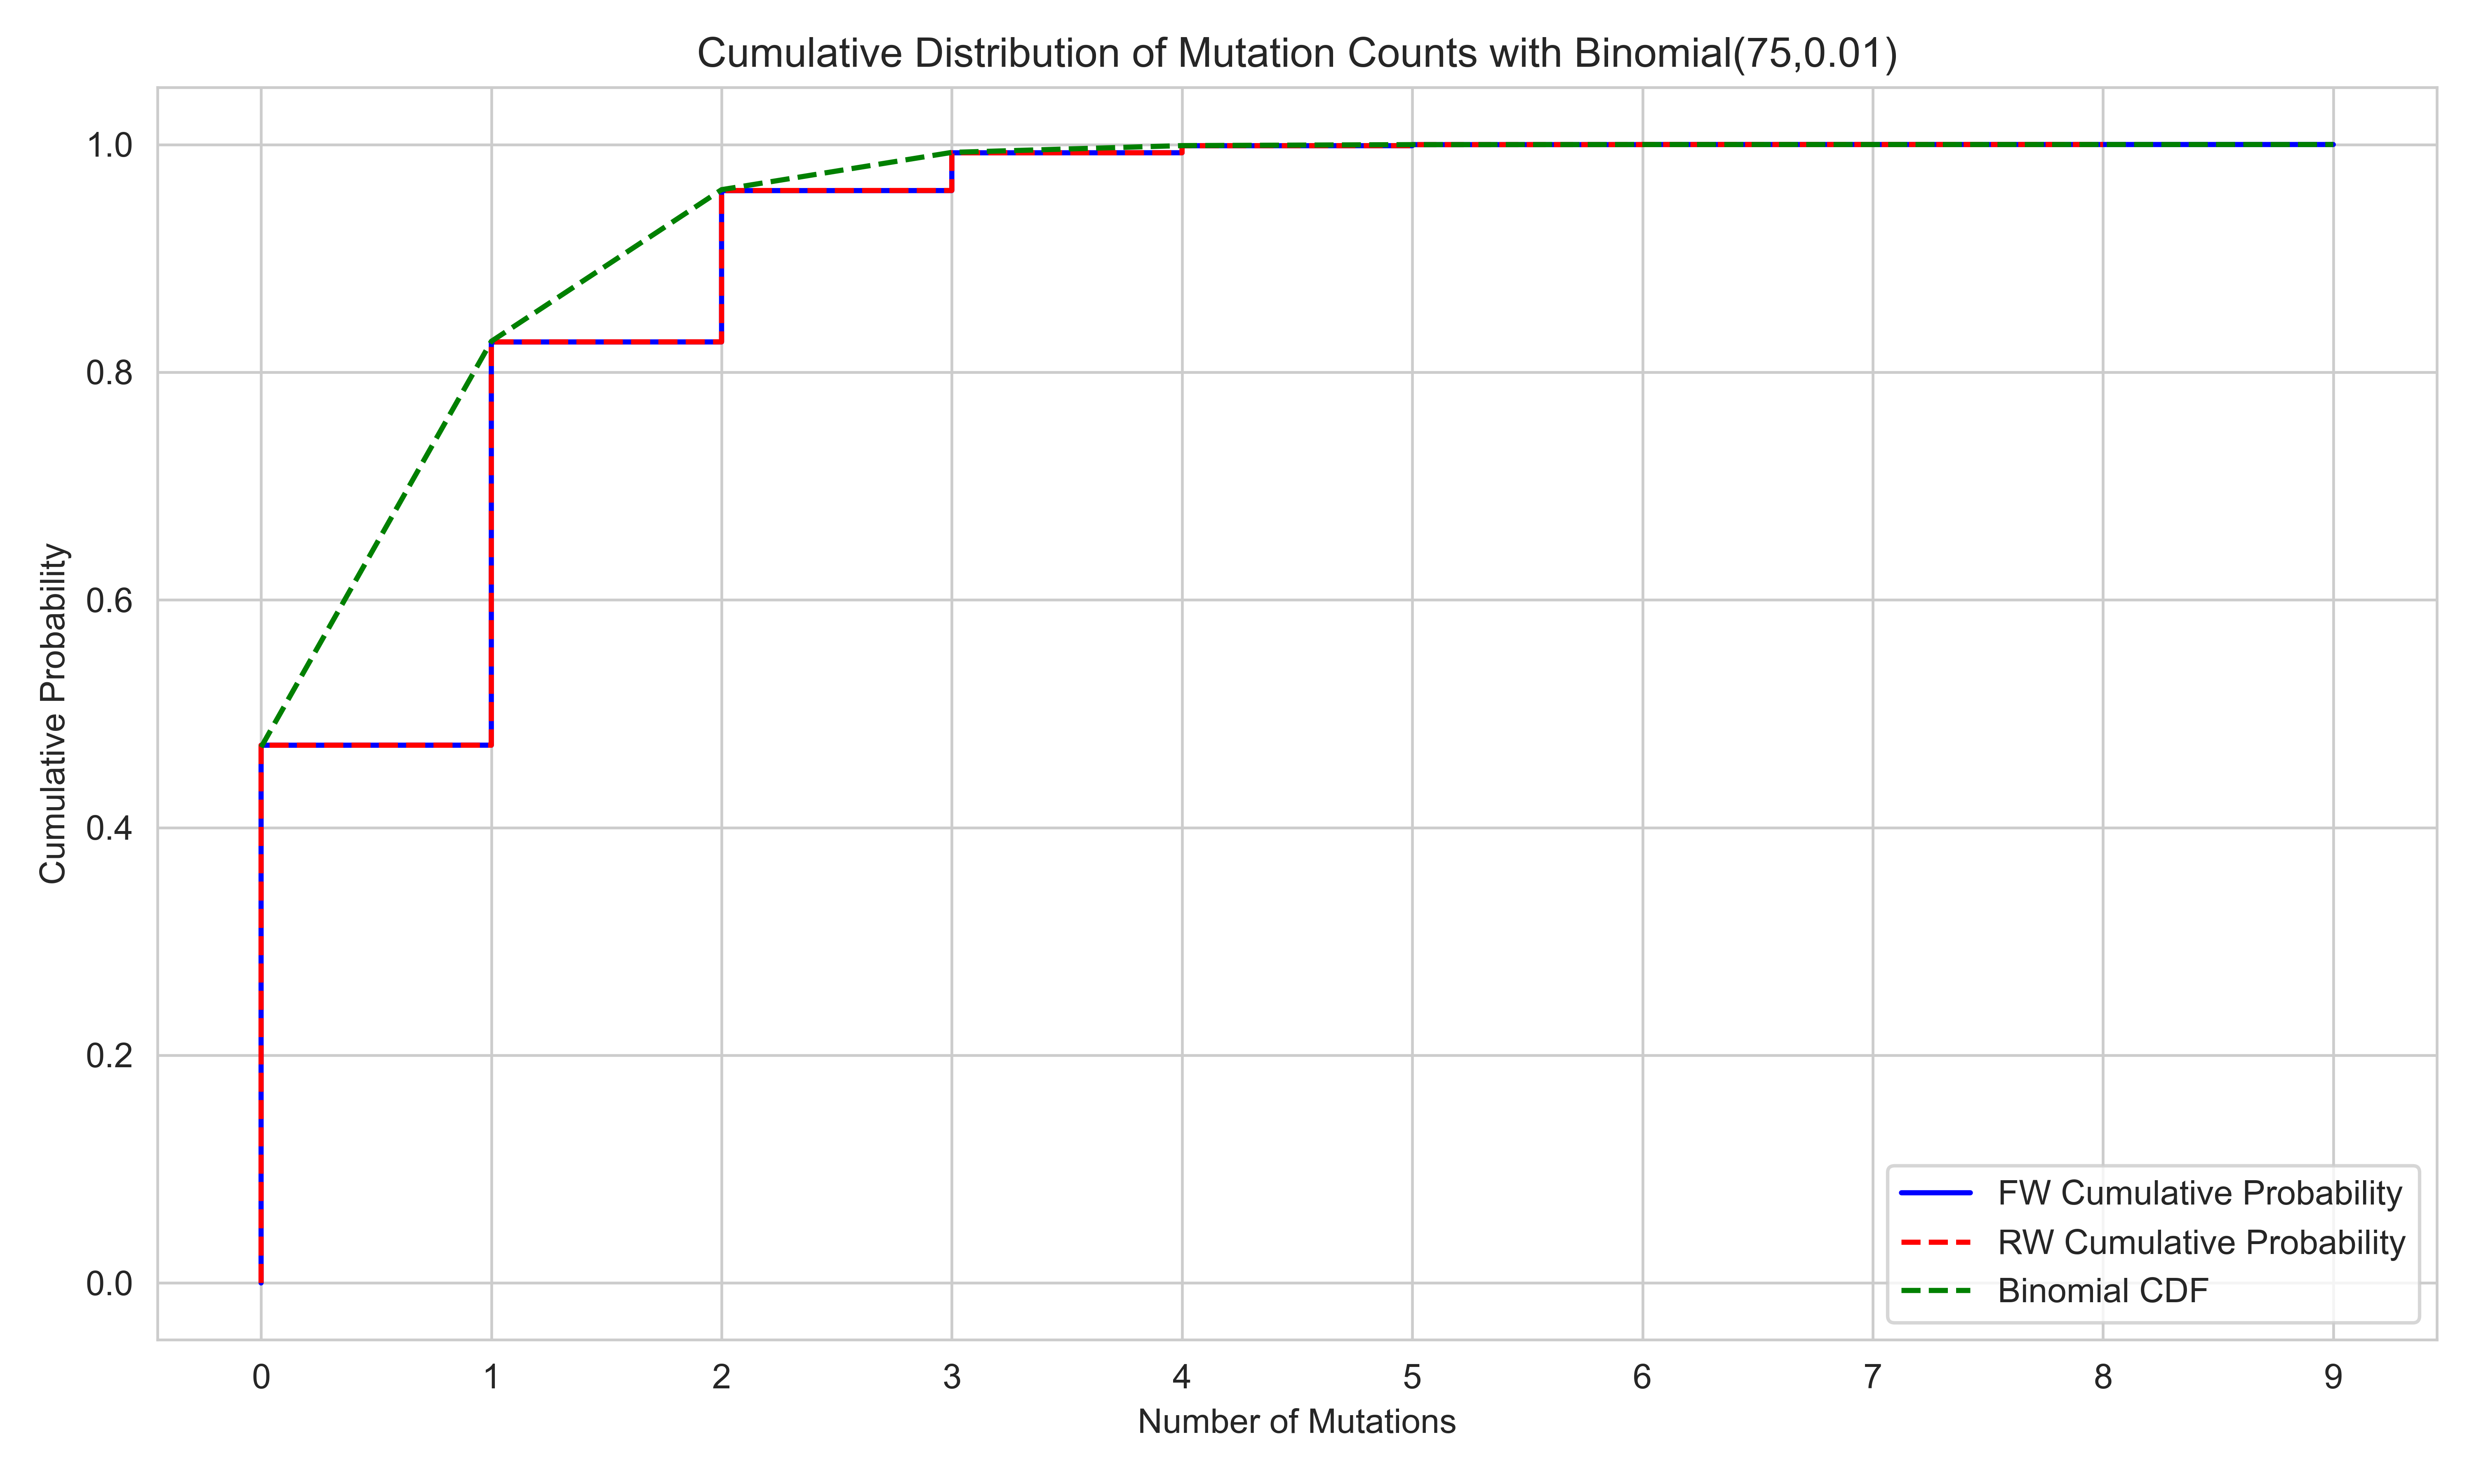
\includegraphics[width=0.7\textwidth]{figures/readsimulator/cumulative_distribution_mutation_counts_FWRW}
        \caption{Cumulative Distribution of mutation counts overlayed with the CDF of binomial(75,0.01)}
        \label{fig:cumulative-distribution-mutation-counts}
    \end{figure}

    \begin{figure}
        \centering
        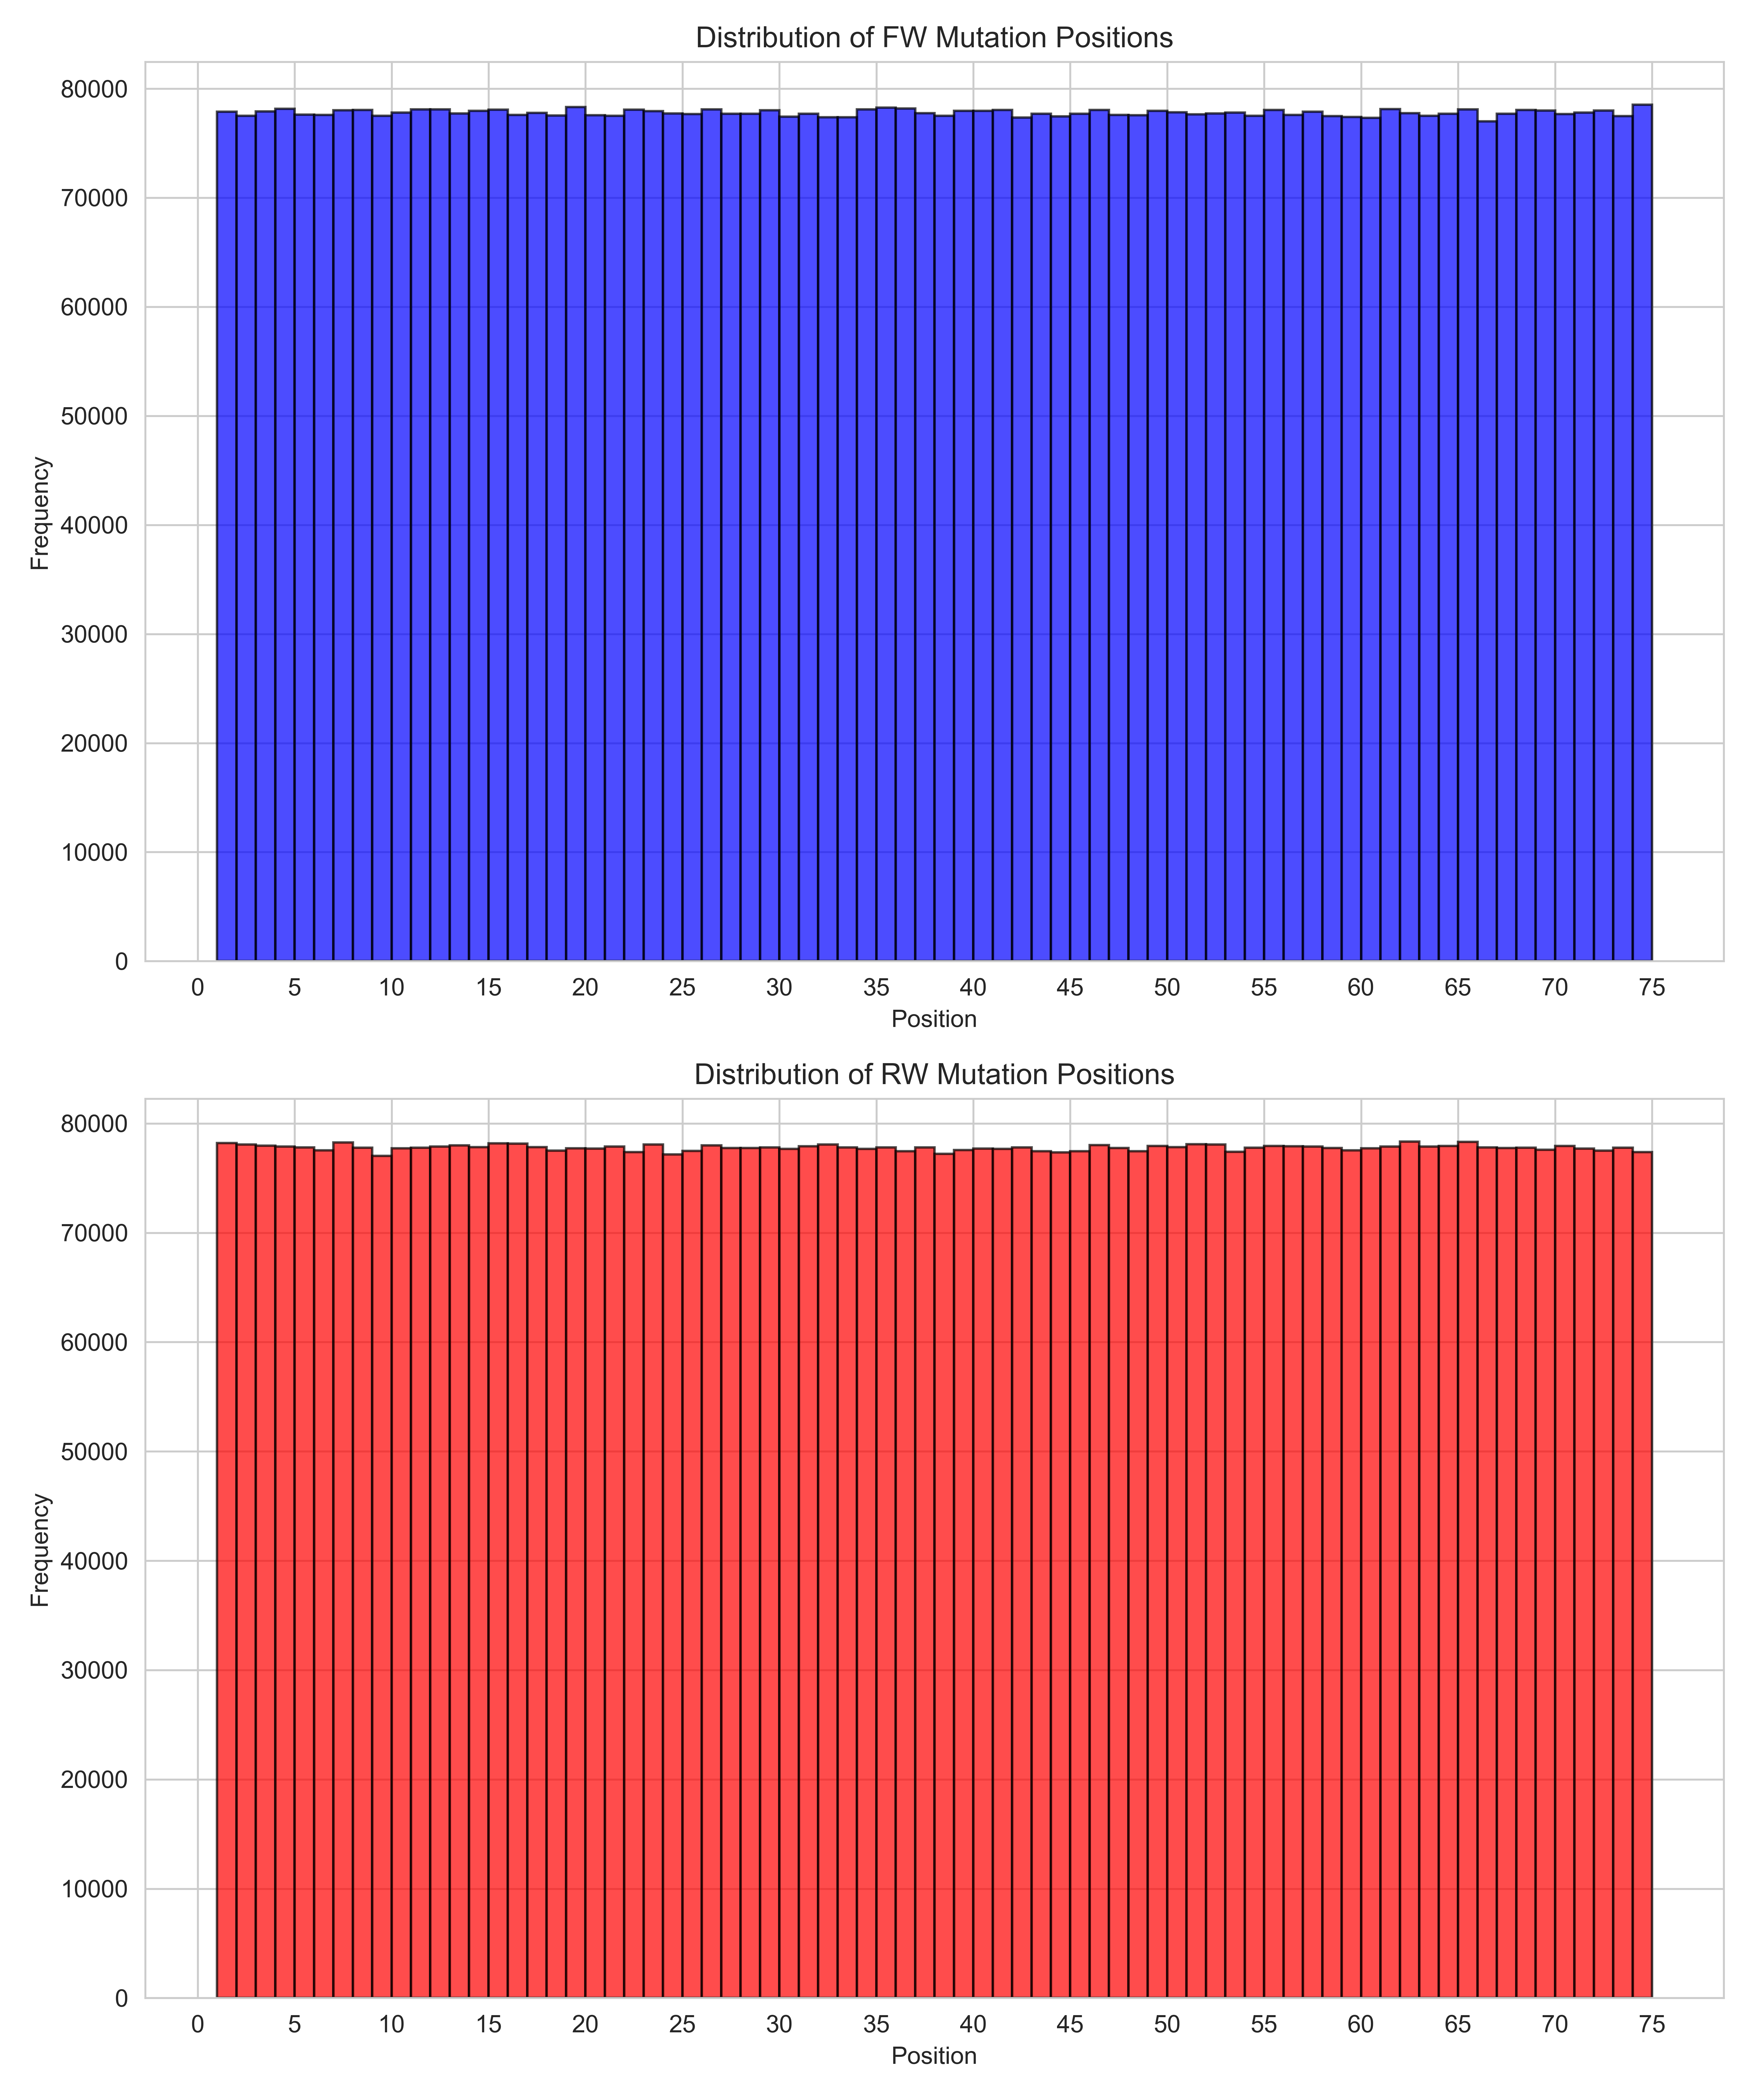
\includegraphics[width=0.5\textwidth]{figures/readsimulator/histogram_mutation_positions}
        \caption{Histogram of the of the positions of mutations}
        \label{fig:histogram_mutation_positions}
    \end{figure}

    \subsubsection{Simulation}

    The \texttt{-analysis-script} option lets users specify the path to the provided analysis script in the submission folder. This script facilitates the creation of comprehensive simulation reports, generating an HTML and PDF file (and saving the plots individually) called \texttt{plots.[pdf,html]}. The analysis output includes four key visualizations:

    \begin{enumerate}
        \item \textbf{Fragment Length Distribution}: A histogram showing the distribution of fragment lengths with mean and standard deviation highlighted.
        \item \textbf{Cumulative Distribution of Mutation Counts}: A cumulative distribution function (CDF) plot comparing forward and reverse mutations alongside a binomial distribution for reference.
        \item \textbf{Read Metrics Bar Plot}: A bar plot illustrating various metrics related to the reads
        \item \textbf{Mutation Position Histogram}: A histogram displaying the frequency of mutation positions across the read sequence.
    \end{enumerate}

    This functionality allows users to efficiently analyze read simulation results, easily identifying any discrepancies or anomalies.

    \subsubsection{Fragment Length}
    The mean fragment length is 200, with a standard deviation of 80. As shown in Figure \ref{fig:fragment-length-dist}, the distribution of fragment lengths exhibits a rightward drift. This drift is attributed to the minimum fragment length constraint of 75, which aligns with the minimum read length. Because we redraw the fragment length if it is smaller than the read length, we naturally see a slight drift of the normal distribution to the right.


    \begin{figure}
        \centering
        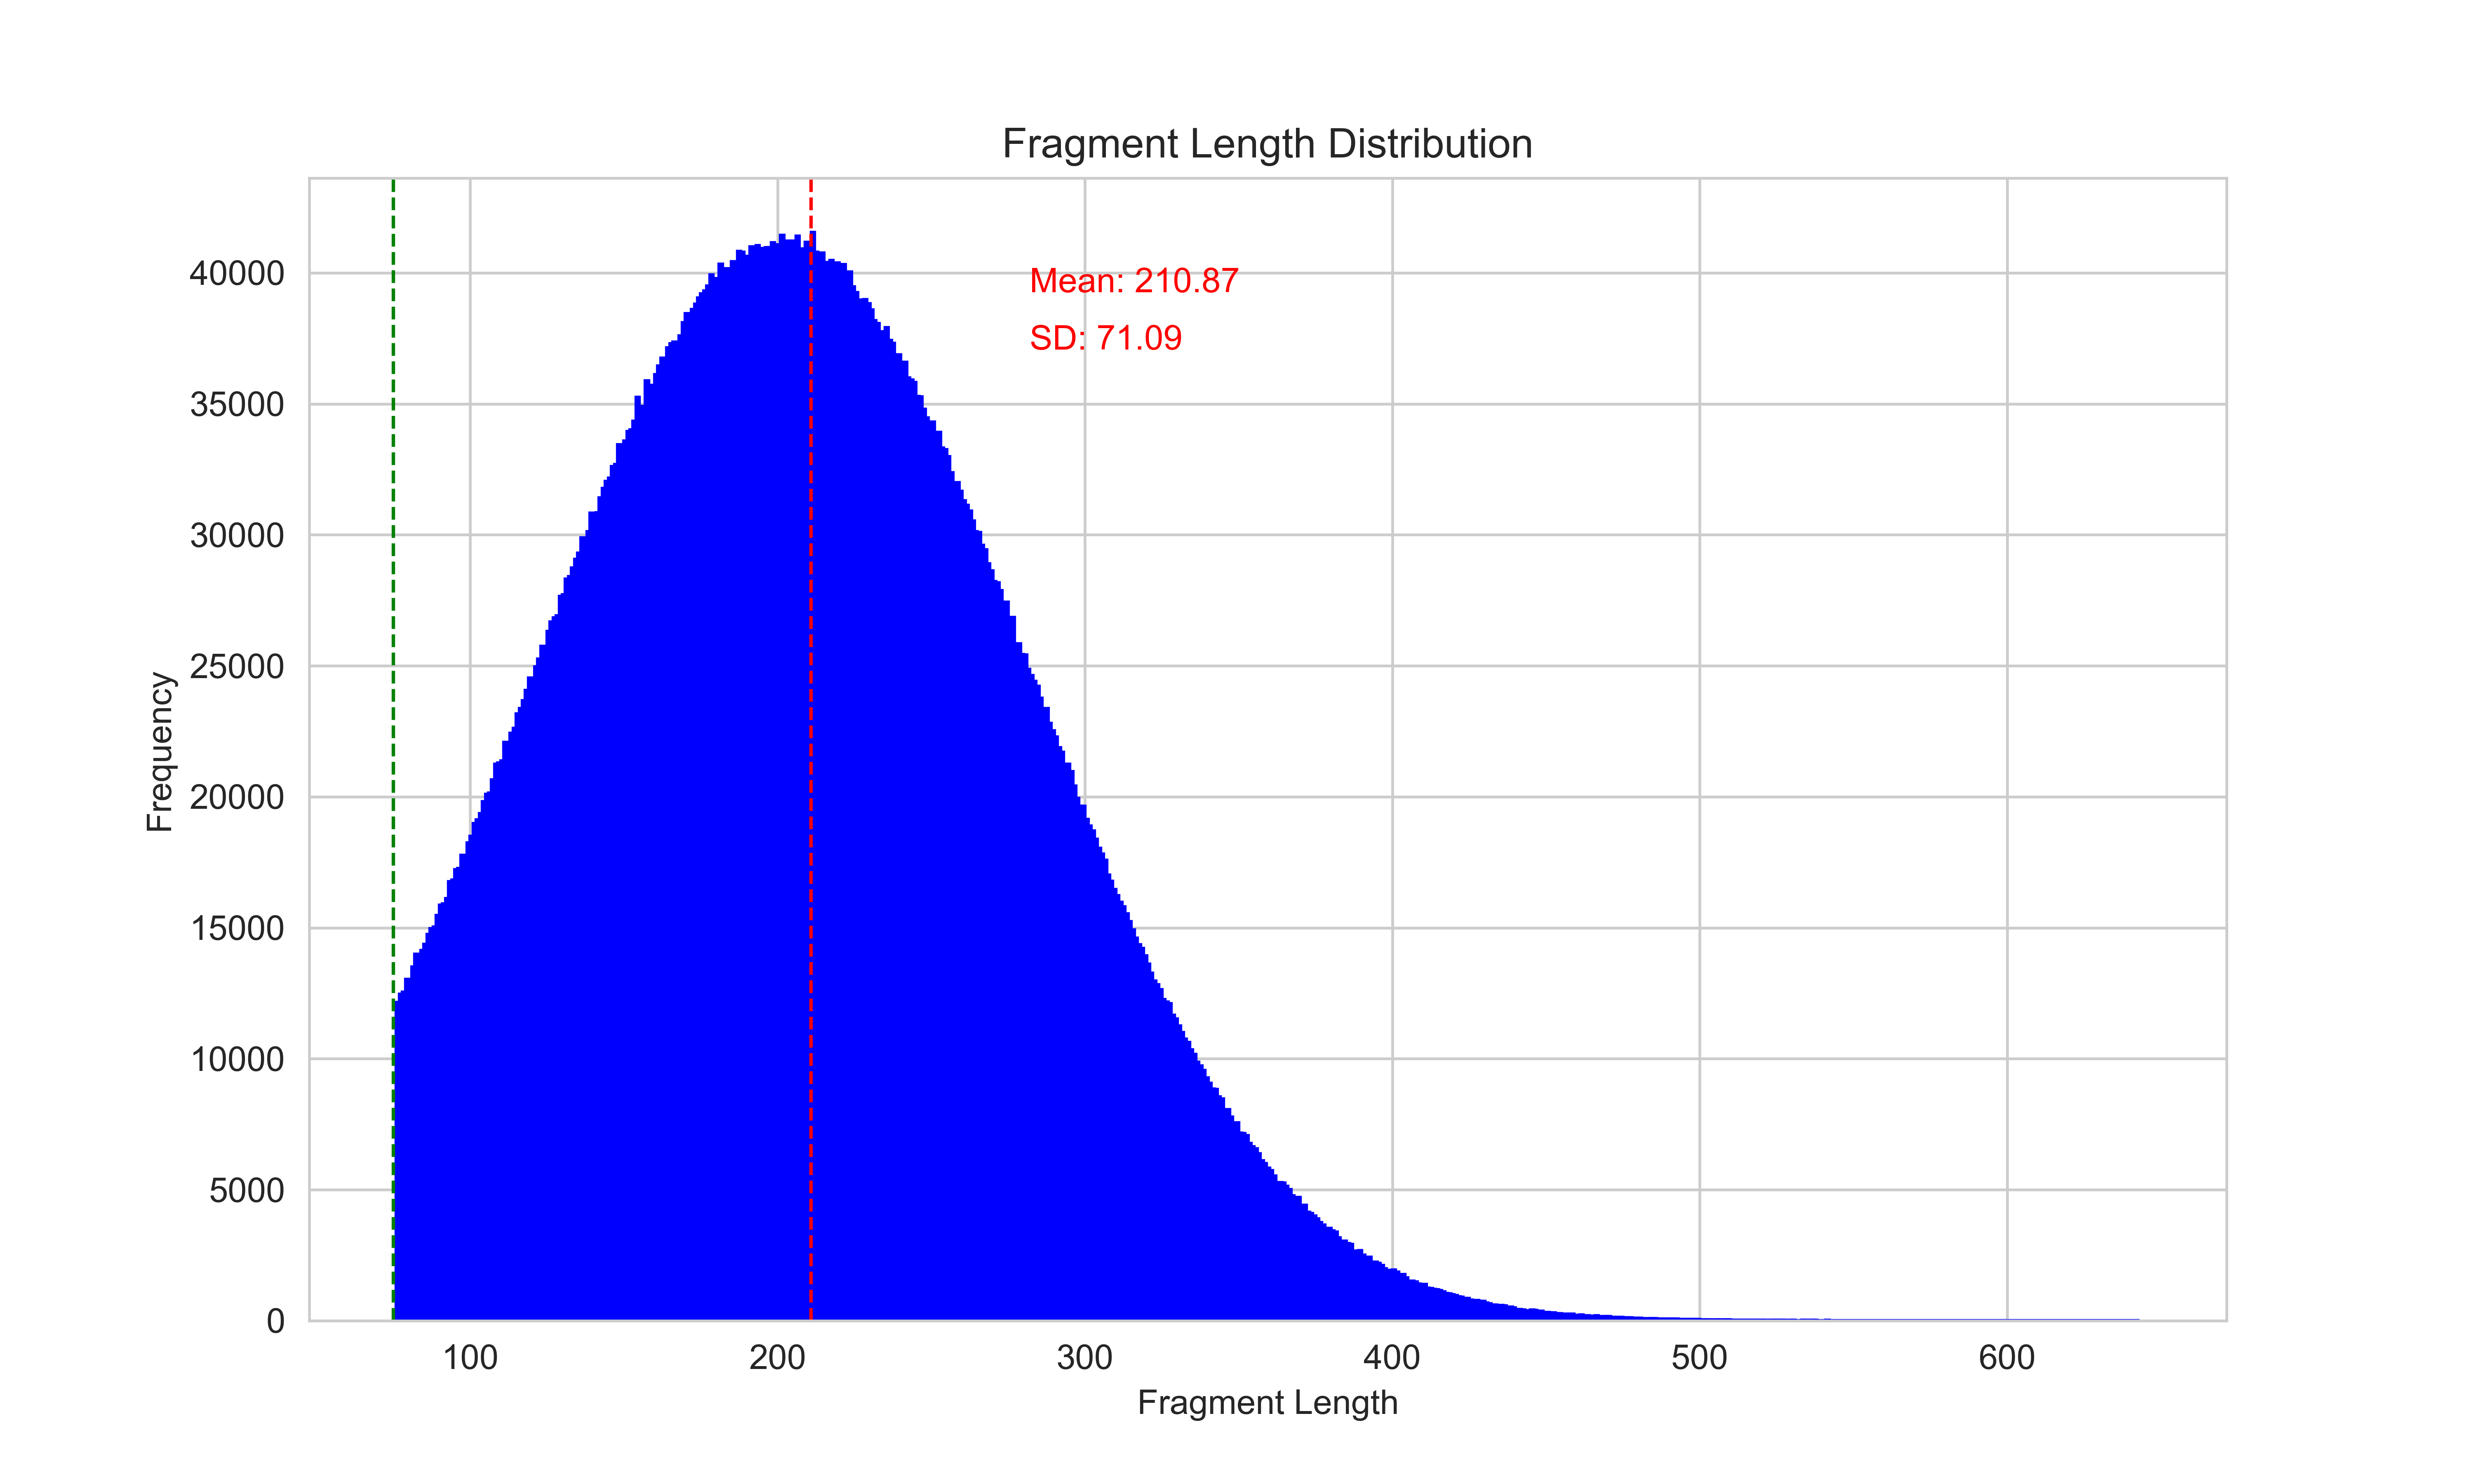
\includegraphics[width=0.7\textwidth]{figures/readsimulator/fragment_length_distribution}
        \caption{Distribution of the Fragment Lengths}
        \label{fig:fragment-length-dist}
    \end{figure}

    \subsubsection{Read Bar Plot}


    The barplot presents the distribution of reads across several categories, providing insights into the characteristics of the sequencing data. The categories analyzed include:

    \begin{itemize}
        \item \textbf{All Reads}: This category represents the total number of reads generated during sequencing. It serves as the baseline for understanding the overall data output.

        \item \textbf{Non-Split Reads}: These reads correspond to genomic regions that consist of a single continuous segment. The count of non-split reads (both forward and reverse) indicates the proportion of reads that do not span multiple regions, which can simplify mapping.

        \item \textbf{Non-Split Reads with No Mismatches}: This subset of non-split reads highlights those that align perfectly to the reference genome.

        \item \textbf{Split Reads}: Split reads are those that span multiple genomic regions.

        \item \textbf{Split Reads with No Mismatches}: This category focuses on split reads that align without any mismatches.

        \item \textbf{Split Reads with No Mismatches (All Regions $\geq$ 5 bp)}: This final category filters split reads to include only those where all regions are at least 5 base pairs long. This criterion excludes reads, which would be difficult to map as they contain only a very short section in one exon.
    \end{itemize}

    Figure \ref{fig:read-bar-plot} displays the selected reads from the sample input, but the absolute quantities or relative distributions do not necessarily have a clear biological significance. Interestingly, forward reads were slightly more likely to be split compared to reverse reads. However, this observation may result from chance related to the specific transcripts chosen. If the transcript chosen only has a few exons, the amount of split reads will also be lower. Similarly, the smaller the read length/fragment length, the lower the chance that a read will surpass the gap between exons. Assuming that our chosen genes and transcripts we generated reads for are generally representative, we can use the distribution to verify that our mapped reads match this distribution. Since our read length of 75 is quite short, this distribution is quite likely, as the average exon is much larger, lowering the chance that a read goes over an intron.

    \begin{figure}
        \centering
        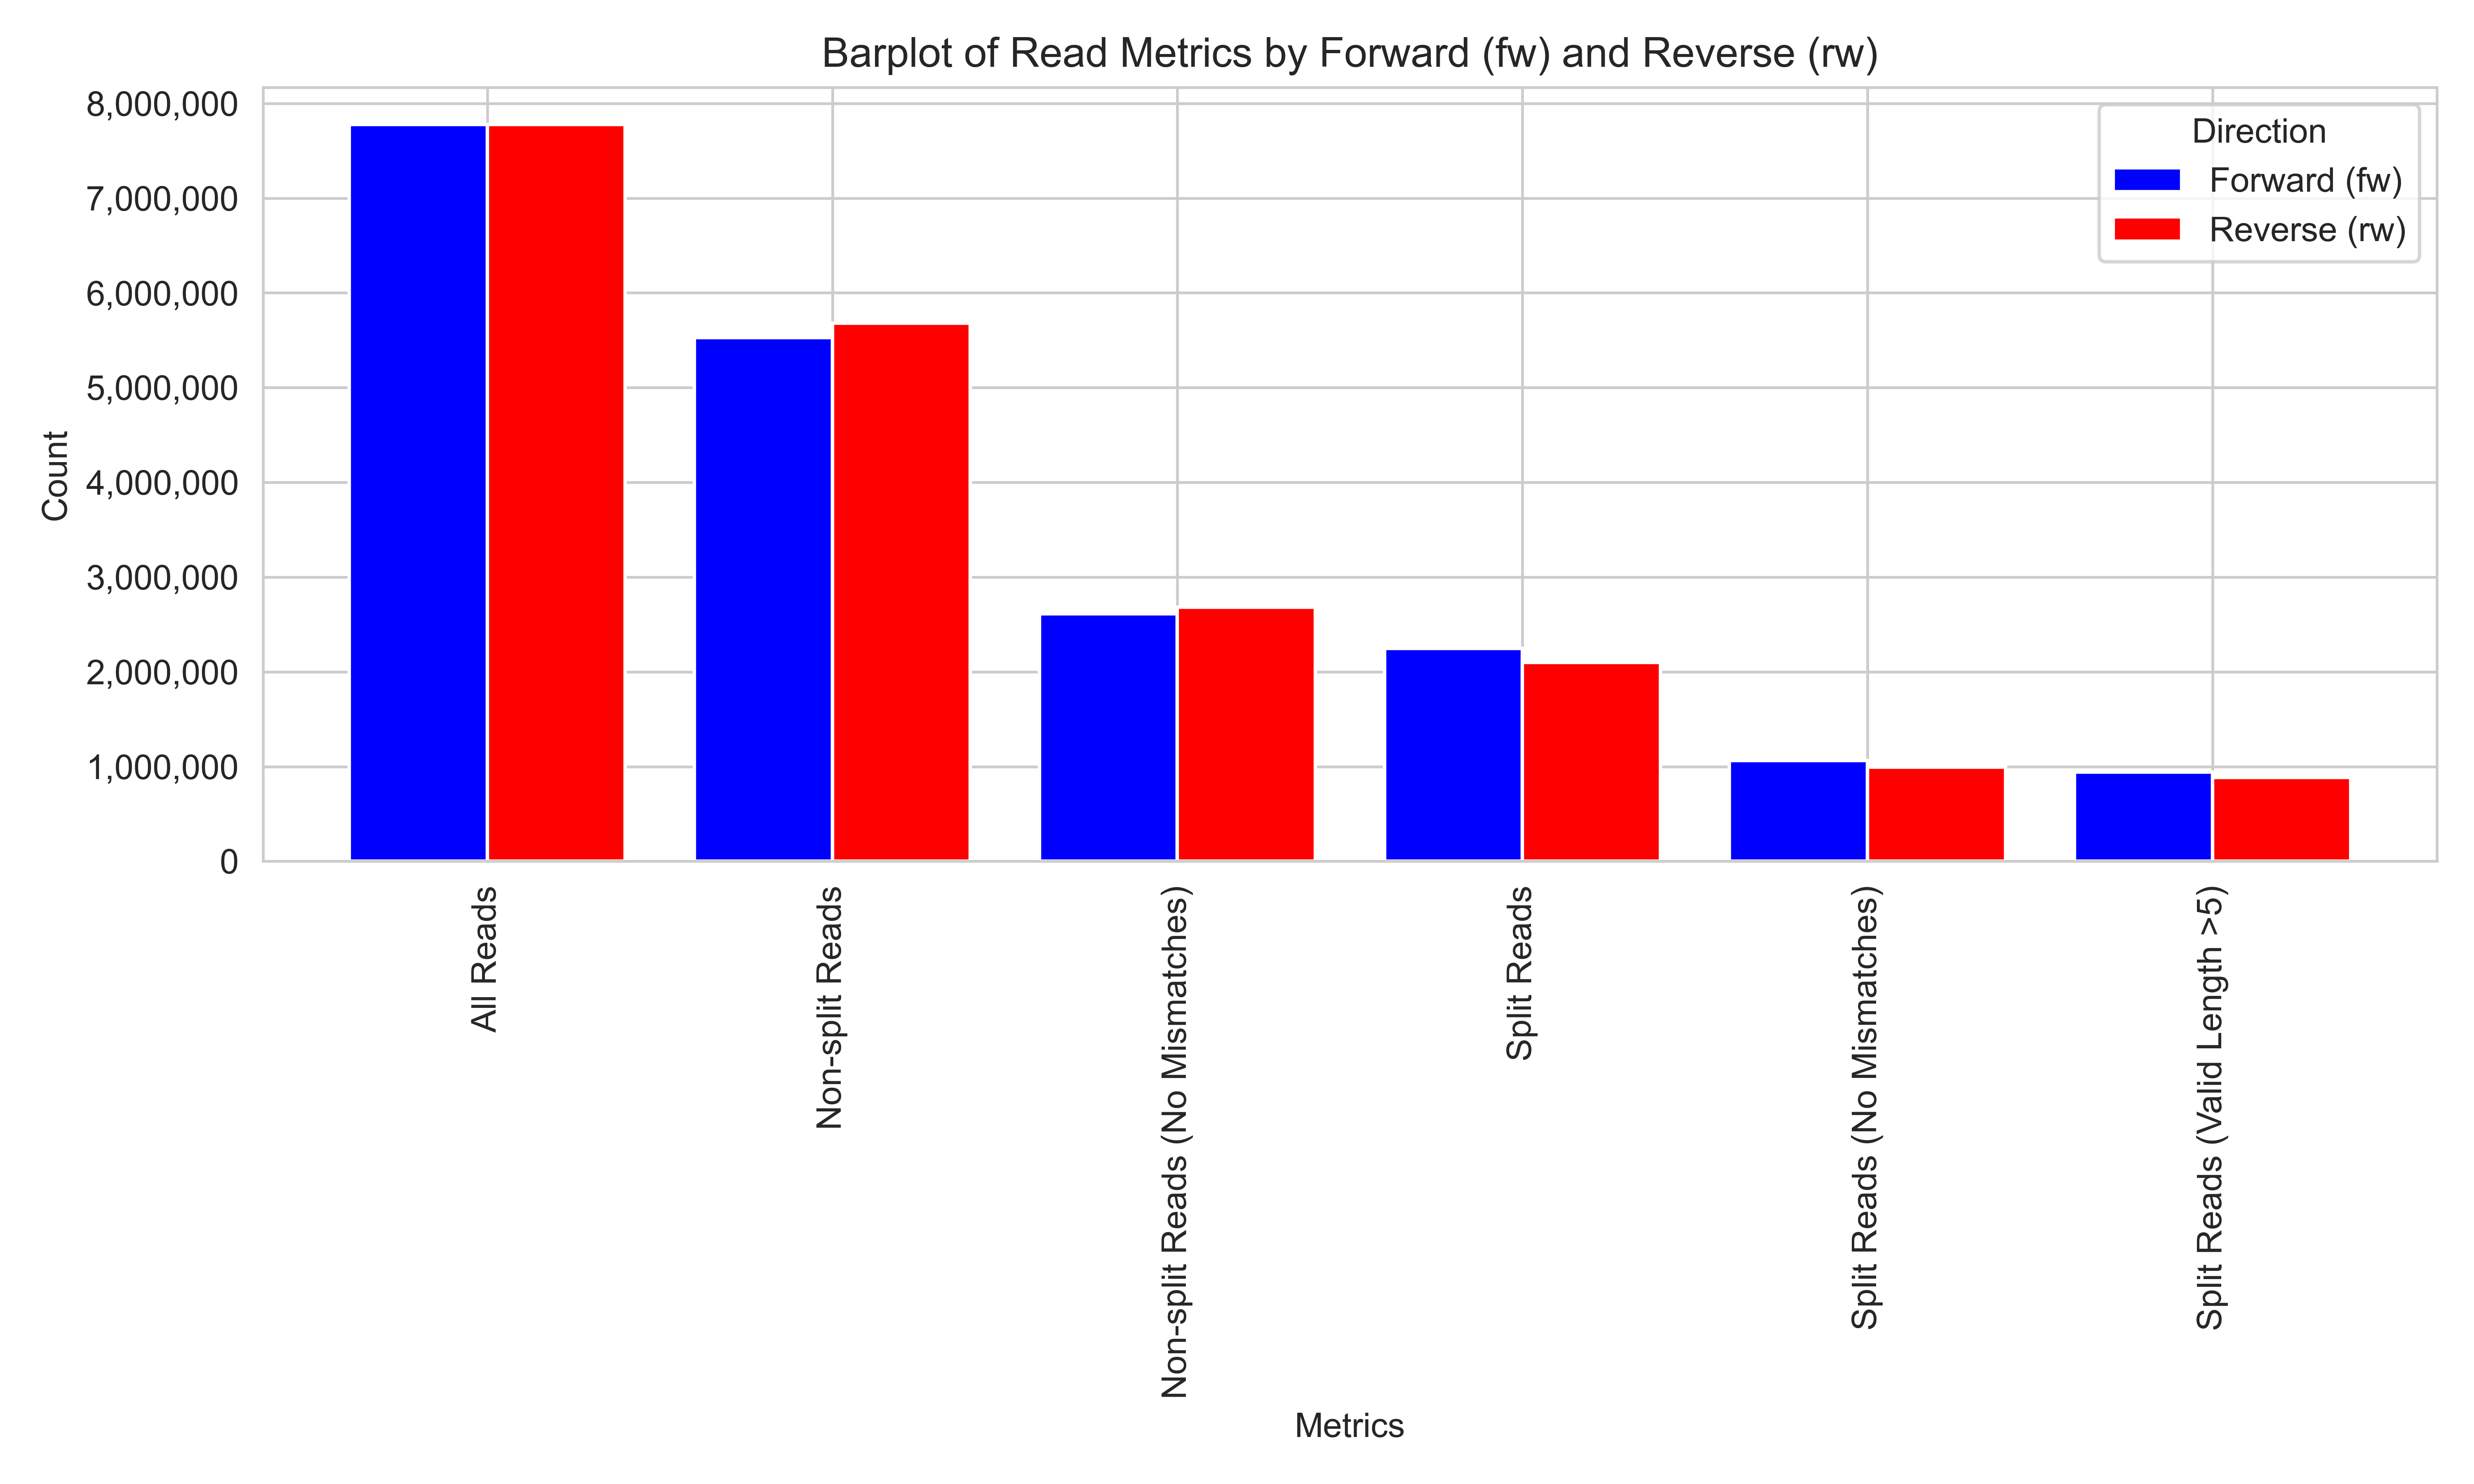
\includegraphics[width=0.7\textwidth]{figures/readsimulator/barplot_read_metrics}
        \caption{Distribution of the Fragment Lengths}
        \label{fig:read-bar-plot}
    \end{figure}

    \subsection{Time}

    \subsubsection{Runtime}
    Tests were conducted on an idle computer with an M2 CPU, 16 GB RAM, and an SSD to benchmark the program's runtime. The program was executed 10 times under these conditions. Timing variables were introduced to gain insights into the proportion of runtime consumed by each major section of the program. These variables measured the duration of key sections as follows:

    \begin{enumerate}
        \item \textbf{Initialization Time}: The time taken to read the read counts and parse the GTF file.
        \item \textbf{Sequence Extraction Time}: The cumulative time spent extracting each sequence from the FASTA file.
        \item \textbf{Fragment Length Sampling Time}: The cumulative time required to sample random fragment lengths.
        \item \textbf{Read Creation Time}: The cumulative time spent creating reads by extracting the fragment.
        \item \textbf{Mutation Time}: The cumulative time needed to introduce mutations into the sequence.
        \item \textbf{Genomic Position Calculation Time}: The cumulative time required to calculate the original genomic region vector for each read.
        \item \textbf{Mapping Info Writing Time}: The cumulative time taken to write information to the mapping info file.
        \item \textbf{FASTQ Writing Time}: The cumulative time used to write the forward and reverse reads to the FASTQ files.
        \item \textbf{Total Read Simulation Time}: The overall time spent running the \texttt{simulate()} method.
        \item \textbf{Total Time}: The total runtime of the entire program.
    \end{enumerate}

    Sections 2 through 8 involve operations executed repeatedly, once for each read. To track these, the \texttt{System.currentTimeMillis()} method was invoked at each step, and the time difference was added to a cumulative total for each section. This introduces additional complexity and likely increases the overall runtime. Thus, these measurements are best interpreted as relative indicators of how long each section contributes to the total runtime rather than absolute measures.

    \begin{figure}
        \centering
        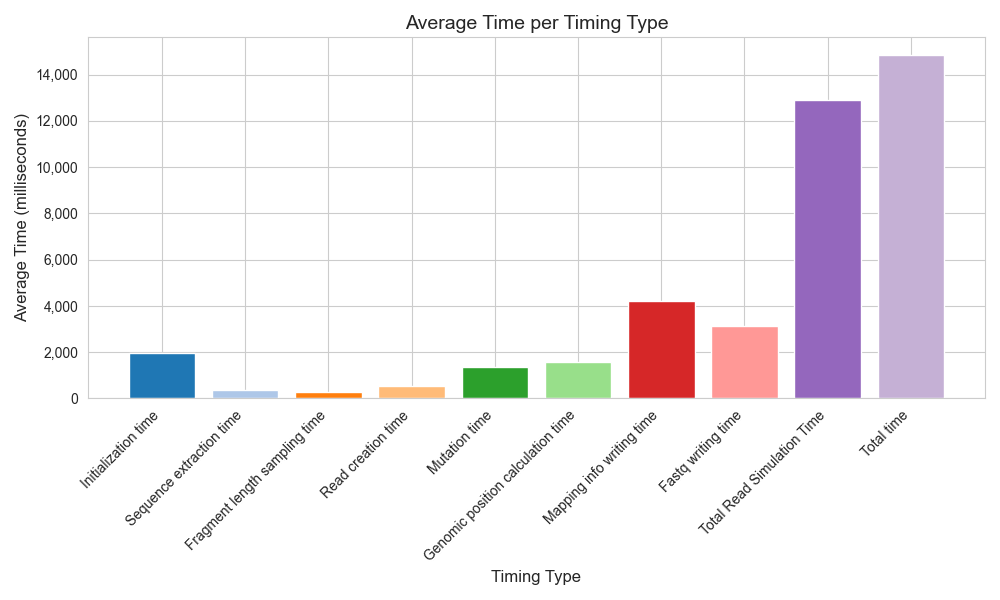
\includegraphics[width=0.7\textwidth]{figures/readsimulator/average_time_per_timing_type}
        \caption{Average runtime for different sections over 10 runs on a computer with M2 CPU, 16GB RAM, and an SSD}
        \label{fig:runtime}
    \end{figure}


    \begin{table}[]
        \caption{Average runtime for different sections over 10 runs on a computer with M2 CPU, 16GB RAM, and an SSD}
        \label{tab:untime}
        \resizebox{\textwidth}{!}{%
            \begin{tabular}{|l|c|c|}
                \hline
                \rowcolor[HTML]{C0C0C0}
                \textbf{Timing Type}              & \multicolumn{1}{l|}{\cellcolor[HTML]{C0C0C0}\textbf{Average Time (ms)}} & \multicolumn{1}{l|}{\cellcolor[HTML]{C0C0C0}\textbf{Proportion of Total Time (\%)}} \\ \hline
                Initialization time               & 1,950                                                                   & 13.12\%                                                                             \\ \hline
                \rowcolor[HTML]{EFEFEF}
                Sequence extraction time          & 376                                                                     & 2.53\%                                                                              \\ \hline
                Fragment length sampling time     & 265                                                                     & 1.78\%                                                                              \\ \hline
                \rowcolor[HTML]{EFEFEF}
                Read creation time                & 545                                                                     & 3.67\%                                                                              \\ \hline
                Mutation time                     & 1,357                                                                   & 9.13\%                                                                              \\ \hline
                \rowcolor[HTML]{EFEFEF}
                Genomic position calculation time & 1,562                                                                   & 10.51\%                                                                             \\ \hline
                Mapping info writing time         & 4,193                                                                   & 28.21\%                                                                             \\ \hline
                \rowcolor[HTML]{EFEFEF}
                FASTQ writing time                & 3,145                                                                   & 21.16\%                                                                             \\ \hline
                Total Read Simulation Time        & 12,911                                                                  & 86.86\%                                                                             \\ \hline
                \rowcolor[HTML]{EFEFEF}
                Total time                        & 14,864                                                                  & 100\%                                                                               \\ \hline
            \end{tabular}%
        }
    \end{table}

    It is important to note that a run without the added timing calculation was conducted for comparison, yielding a total runtime of \emph{12,444ms}. Additionally, since \texttt{currentTimeMillis()} rounds to the nearest millisecond, any section taking less than 1 millisecond (e.g., 0.4ms) would be recorded as 0ms, potentially underestimating the actual time for very short operations. Another critical point is that since the GTF annotation file is only parsed once at the beginning during the initialization phase, the proportion of time spent on initialization decreases as the number of reads generated increases. This means that for larger datasets, the relative impact of the initialization time diminishes.


    Sections 2 through 8 do not encompass all operations within the \texttt{simulate()} method; for example, they exclude minor operations like iterating over reads to be simulated and other small overhead tasks. Consequently, the total read simulation time is expected to be slightly higher than the sum of times reported for these sections.

    Table \ref{tab:untime} and Figure \ref{fig:runtime} show this experiment's results. The most intensive part of the simulation is the \texttt{FASTQ writing time} and \texttt{Mapping info writing time}. This is to be expected as we are writing quite large files. The \texttt{Mutation time} and \texttt{Genomic Position Calculation} also contribute significantly, at 9.13\% (1,357 ms) and 10.51\% (1,562 ms), respectively. These include string operations like taking the reverse complement and sampling the poisson distribution to simulate the mutations. In contrast, the least time-consuming processes are the \texttt{Sequence extraction time} and \texttt{Fragment length sampling time}, which account for only 2.53\% (376 ms) and 1.78\% (265 ms) of the total time, respectively. If the individual segments of the Read Simulation are added together, they miss 1,468ms of the Total Read Simulation Time. As stated previously, this represents the miscellaneous tasks such as iterating through the Readcounts HashMap and the timing variables, which need to be updated and check the system time in every read.

    \subsubsection{Complexity}
    For this analysis, we will be examining the worst-case performance of the read simulation, excluding any initialization steps for the GTF annotation and read counts, as these remain unchanged regardless of the number of reads we want to simulate. The program's runtime primarily depends on the number of reads, denoted as \( m \) from here on. The worst-case scenario occurs when each read originates from a different transcript, requiring the extraction of a unique transcript sequence for each read. Furthermore, this scenario assumes all transcripts are located on the reverse strand, necessitating an additional step to compute the reverse complement.

    We can express the operations performed by the read simulator in the following equation:
    \[
        m \cdot (t + t + 1 + r + 2r + 2e + 2r)
    \]
    where:
    \begin{itemize}
        \item \( t \): Maximum transcript length
        \item \( e \): Number of exons, where \( e \ll t \)
        \item \( r \): Read length
    \end{itemize}

    For each read we simulate, the operations can be broken down as follows:

    \begin{enumerate}
        \item \textbf{Transcript Reading}: Reading the transcript sequence, proportional to the transcript length \( t \).
        \item \textbf{Reverse Complement Calculation}: Computing the reverse complement of the transcript, also proportional to the transcript length \( t \).
        \item \textbf{Fragment Length and Start Position Sampling}: A constant-time operation, independent of transcript or read length.
        \item \textbf{Forward Read Extraction}: Taking a substring of the transcript sequence, proportional to the read length \( r \).
        \item \textbf{Reverse Read Extraction and Reverse Complement}: Taking a substring for the reverse read and computing its reverse complement, both proportional to the read length \( r \).
        \item \textbf{Mutation Application}: Mutating both reads, an operation proportional to the read length \( r \).
        \item \textbf{Genomic Coordinate Calculation}: Calculating genomic coordinates for both reads. This step involves iterating over all exons and is proportional to the number of exons \( e \).
        \item \textbf{FASTQ Writing}: Writing both reads to the FASTQ files, proportional to the read length \( r \).
    \end{enumerate}

    Since the maximum transcript length \( t \) and the read length \( r \) are constants (as they do not vary with the number of reads \( m \)), we can simplify our complexity analysis. The number of exons \( e \) is also significantly smaller than \( t \), making it negligible for our worst-case approximation. As a result, our equation simplifies, and the runtime of the read simulator is approximately:

    \[
        O(m)
    \]

    where \( m \) is the number of reads to simulate. This linear time complexity reflects the dependency of the program's runtime on the number of reads.


\end{document}
